\section{公共建模内核：守恒型柱坐标耦合场的有限体积求解}\label{sec:kernel}

四个子问题共享同一套守恒律、离散格式与时间推进策略。本节一次性建立这一公共内核，
后续问题章只在此基础上说明"保留了什么、新增了什么、结果如何改变"，不再重复整套推导。
四问在同一内核上的递进关系与总体技术路线见图~\ref{fig:roadmap}。

\begin{figure}[H]
  \centering
  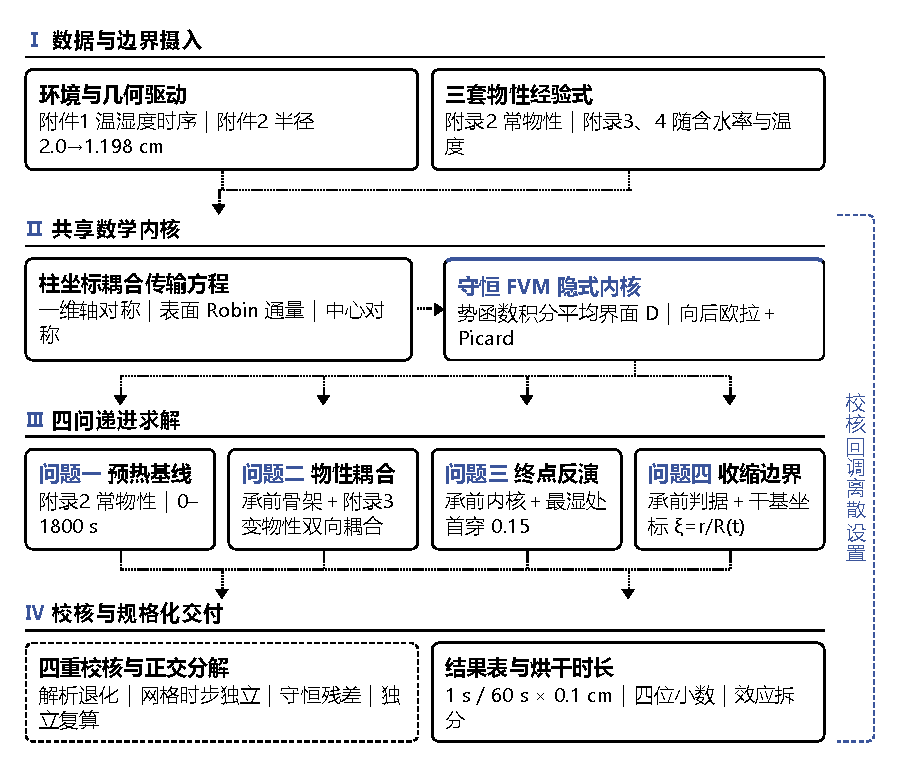
\includegraphics[width=0.94\textwidth,height=0.8\textheight,keepaspectratio]{../figures/fig_roadmap.pdf}
  \caption{总体技术路线：从守恒律到公共数值内核，再逐问增量扩展}
  \label{fig:roadmap}
\end{figure}

图~\ref{fig:roadmap} 表明四问并非彼此独立的四个模型，而是同一守恒型有限体积内核在
"物性—边界—求解域"三个层次上的递进，故各问题章只描述本问新增或改变的部分。

\subsection{控制方程与定解条件}

以柱坐标轴心为原点，取半径 $r\in[0,R_0]$。对任意以轴为中心、半径 $r$ 的同轴圆柱控制面，
能量守恒与水分质量守恒给出通量的散度形式；在轴对称、忽略轴向与周向输运后，得到一对
非稳态抛物型方程：
\begin{equation}\label{eq:pde}
\rho c_p\,\frac{\partial T}{\partial t}=\frac{1}{r}\frac{\partial}{\partial r}\!\left(r\,k\,\frac{\partial T}{\partial r}\right),
\qquad
\frac{\partial C}{\partial t}=\frac{1}{r}\frac{\partial}{\partial r}\!\left(r\,D\,\frac{\partial C}{\partial r}\right),
\qquad 0<r<R_0 .
\end{equation}
式~\eqref{eq:pde} 中左端为单位体积的热/水分储量变化率，右端 $\frac{1}{r}\partial_r(r\,\cdot)$ 是柱坐标下的
散度算子，$k,D$ 分别为导热系数与水分扩散系数。表面 $r=R_0$ 处，内部扩散/导热通量必须与
外部对流带走的水分/热量平衡，得 Robin 边界；轴心 $r=0$ 处由对称性得零通量：
\begin{equation}\label{eq:bc}
\left.-D\frac{\partial C}{\partial r}\right|_{R_0}=h_m\,(C_s-C_{\mathrm{air}}),\quad
\left.-k\frac{\partial T}{\partial r}\right|_{R_0}=h\,(T_s-T_{\mathrm{air}}),\quad
\left.\frac{\partial C}{\partial r}\right|_{0}=\left.\frac{\partial T}{\partial r}\right|_{0}=0 .
\end{equation}
初始条件为 $T(r,0)=T_0=28\,^{\circ}\mathrm{C}$、$C(r,0)=C_0=2.55$。几何与边界条件的对应关系见
图~\ref{fig:tikz_geometry_bc}。

\begin{figure}[H]
  \centering
  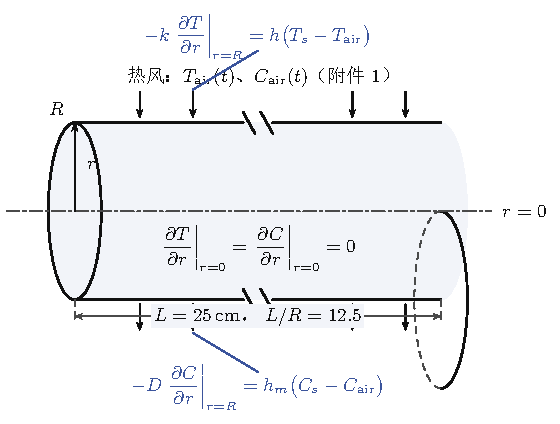
\includegraphics[width=0.9\textwidth,height=0.8\textheight,keepaspectratio]{../figures/tikz_geometry_bc.pdf}
  \caption{圆柱几何与柱坐标边界条件：表面 Robin、轴心零通量、端面忽略}
  \label{fig:tikz_geometry_bc}
\end{figure}

图~\ref{fig:tikz_geometry_bc} 明确了三类边界的物理归属：表面同时承担对流换热与对流传质，
轴心因对称退化为绝热绝湿面，端面则因长径比大而被忽略。式~\eqref{eq:pde}--\eqref{eq:bc}
是四问共用的连续模型，各问的差异仅在于 $\rho,c_p,k,D$ 与 $T_{\mathrm{air}},C_{\mathrm{air}}$ 的具体形式。
热量与水分的输运路径见图~\ref{fig:scene}。

\begin{figure}[H]
  \centering
  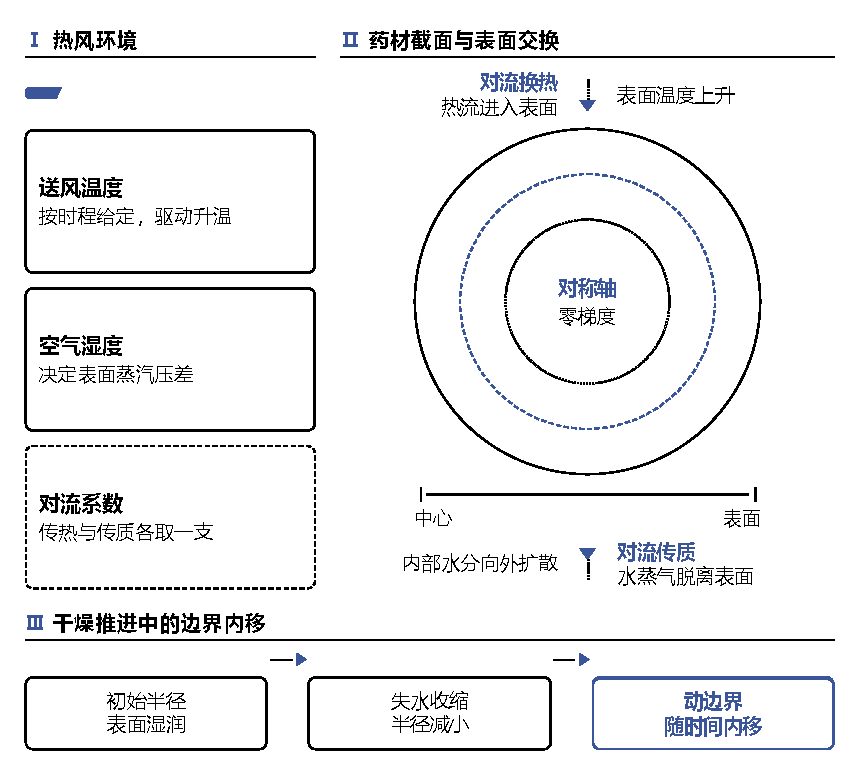
\includegraphics[width=0.92\textwidth,height=0.8\textheight,keepaspectratio]{../figures/fig_scene.pdf}
  \caption{热风烘干中的表面对流换热、对流传质与内部径向扩散}
  \label{fig:scene}
\end{figure}

图~\ref{fig:scene} 表明：热风以对流换热系数 $h$ 向表面供热，水分以对流传质系数 $h_m$
从表面逸出，内部则由导热与扩散把边界扰动向轴心传播；轴心响应最慢，是"内部各点均达标"
判据的控制点。

\subsection{三套物性与扩散系数的量级差异}

三套附录给出的物性形式不同：附录2 为常物性；附录3、附录4 均取
$\rho=\rho_0+\rho_1 C$、$c_p=c_{p0}+c_{p1}\frac{C}{C+1}$、$k=k_0+k_1\frac{C}{C+1}$，扩散系数则统一采用
Arrhenius 型
\begin{equation}\label{eq:diff}
D(C,T)=D_0\,\exp\!\left(-\frac{a}{C}\right)\exp\!\left(-\frac{E}{T_K}\right),\qquad T_K=T+273.15 ,
\end{equation}
其中 $\exp(-a/C)$ 刻画低含水率时自由水减少导致的扩散受阻，$\exp(-E/T_K)$ 为温度激活项，
$E=3850\,\mathrm{K}$\upcite{tong1990,ma2026}。附录3 取 $D_0=2.4\times10^{-3},a=0.45$，附录4 取
$D_0=4.2\times10^{-4},a=0.30$，各附录完整物性见表~\ref{tab:properties}。三套扩散系数的量级
对比与附录3 的二维响应面见图~\ref{fig:diffusivity_range} 与图~\ref{fig:diffusivity_contour}。

% 表：三套附录物性模型与关键参数
% 数据来源：PROBLEM_FACTS.json → code/params.py（OCR SHA256 核验）
\begin{table}[H]
  \centering
  \caption{三套附录物性模型对照}
  \label{tab:properties}
  \small
  \begin{tabular}{llll}
    \toprule
    物性量 & 附录2（问题1） & 附录3（问题2、3） & 附录4（问题4） \\
    \midrule
    密度 $\rho$ / (kg$\cdot$m$^{-3}$)
      & $820$
      & $650+128\,C$
      & $760+90\,C$ \\
    比热 $c_p$ / (J$\cdot$kg$^{-1}$K$^{-1}$)
      & $2600$
      & $1450+2736\dfrac{C}{C+1}$
      & $1850+2150\dfrac{C}{C+1}$ \\
    导热 $k$ / (W$\cdot$m$^{-1}$K$^{-1}$)
      & $0.36$
      & $0.21+0.38\dfrac{C}{C+1}$
      & $0.12+0.20\dfrac{C}{C+1}$ \\
    扩散系数 $D$ / (m$^2\cdot$s$^{-1}$)
      & $7{\times}10^{-9}e^{-0.89/C}$
      & $2.4{\times}10^{-3}e^{-0.45/C}e^{-3850/T_K}$
      & $4.2{\times}10^{-4}e^{-0.30/C}e^{-3850/T_K}$ \\
    \midrule
    $D$ 初始值（$C_0$，$28^\circ$C）
      & $4.938{\times}10^{-9}$
      & $5.642{\times}10^{-9}$
      & 随工况 \\
    $D$ 终点值（$C_{\rm th}$，$50^\circ$C）
      & ---
      & $8.001{\times}10^{-10}$
      & 随工况 \\
    温度依赖性
      & 无
      & Arrhenius
      & Arrhenius \\
    边界域
      & 固定 $R_0$
      & 固定 $R_0$
      & 动边界 $R(t)$ \\
    \bottomrule
  \end{tabular}

  \vspace{2pt}
  \parbox{0.94\linewidth}{\footnotesize
  注：$C$ 为干基含水率（kg$\cdot$kg$^{-1}$），$T_K$ 为开尔文温度。
  共用参数：$R_0=2$ cm，$L=25$ cm，$T_0=28^\circ$C，$C_0=2.55$，达标阈值
  $C_{\rm th}=0.15$，对流换热 $h=25$ W$\cdot$m$^{-2}$K$^{-1}$，
  对流传质 $h_m=8{\times}10^{-7}$ m$\cdot$s$^{-1}$。
  $D$ 锚点值由上式复算，与题面校核点一致。}
\end{table}


表~\ref{tab:properties} 给出的锚点表明：初始状态 $D(C_0,28\,^{\circ}\mathrm{C})$ 在附录2、附录3
分别为 $4.938\times10^{-9}$ 与 $5.642\times10^{-9}\,\mathrm{m^2/s}$，量级相当；但降到阈值附近
$D(C_{\mathrm{th}},50\,^{\circ}\mathrm{C})$ 骤降至 $8.001\times10^{-10}$，说明干燥末期扩散显著变慢，这正是
干燥曲线后段拖尾的根源。

\begin{figure}[H]
  \centering
  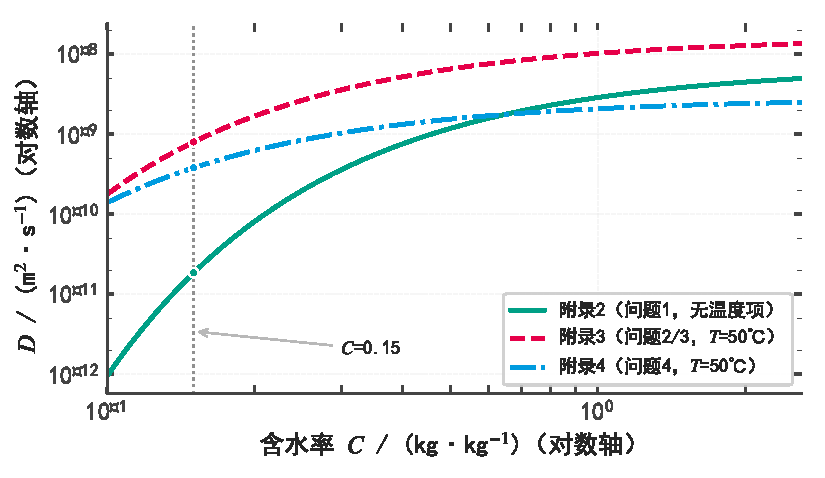
\includegraphics[width=0.9\textwidth,height=0.8\textheight,keepaspectratio]{../figures/fig_diffusivity_range.pdf}
  \caption{三套附录扩散系数在 $C\in[C_{\mathrm{th}},C_0]$ 上的量级对比}
  \label{fig:diffusivity_range}
\end{figure}

图~\ref{fig:diffusivity_range} 显示，随含水率从 $C_0$ 降到 $C_{\mathrm{th}}$，扩散系数跨越约一个数量级，
且三套物性的下降斜率因 $a$ 不同而分化：$a$ 越大（附录2 的等效 $a=0.89$），末期抑制越强。
这一强非线性使得直接对 $D\partial_r C$ 作简单平均会显著失真，必须在离散时对界面扩散通量
作专门处理，详见 \ref{sub:kirchhoff} 节。

\begin{figure}[H]
  \centering
  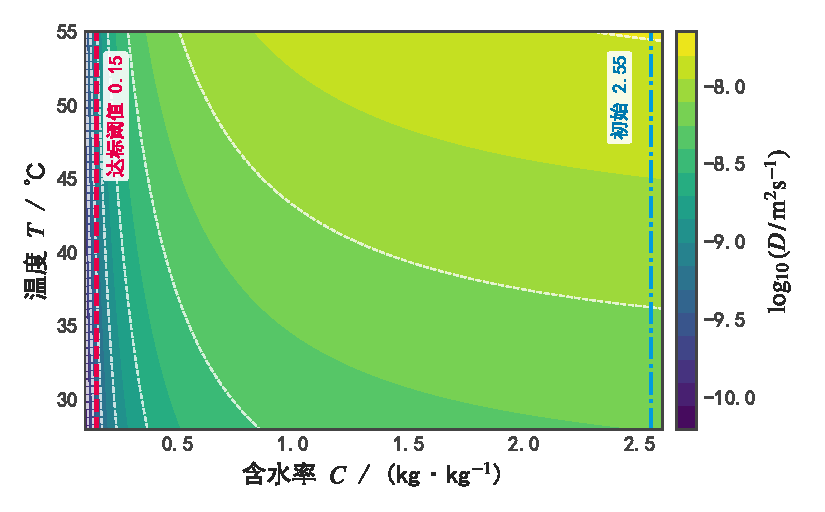
\includegraphics[width=0.9\textwidth,height=0.8\textheight,keepaspectratio]{../figures/fig_diffusivity_contour.pdf}
  \caption{附录3 扩散系数 $D(C,T)$ 在含水率—温度平面上的二维响应面}
  \label{fig:diffusivity_contour}
\end{figure}

图~\ref{fig:diffusivity_contour} 进一步表明 $D$ 对 $C$ 的敏感度远高于对 $T$：等值线沿含水率
方向密集、沿温度方向平缓，说明在本题温区（$28\sim50\,^{\circ}\mathrm{C}$）内，含水率是控制扩散的
主因，温度主要通过 Arrhenius 项作二阶调节。这为问题三、四把终点判据建立在含水率场上
（而非温度场）提供了依据。

\subsection{守恒型有限体积离散}

把 $[0,R_0]$ 划分为 $N$ 个控制体，节点 $r_j$ 位于控制体形心，控制面位于 $r_{j\pm1/2}$。
对式~\eqref{eq:pde} 在第 $j$ 个环形控制体上作体积分，利用散度定理把体积分化为控制面上的
通量差，得到严格守恒的半离散格式（以 $C$ 为例，$T$ 同构）：
\begin{equation}\label{eq:fvm}
w_j\,\frac{\mathrm{d}C_j}{\mathrm{d}t}
=\frac{2}{R_0^2}\Big[\,r_{j+\frac12}\,\widehat{D}_{j+\frac12}\,\frac{C_{j+1}-C_j}{\Delta r}
-\,r_{j-\frac12}\,\widehat{D}_{j-\frac12}\,\frac{C_j-C_{j-1}}{\Delta r}\,\Big],
\qquad
w_j=\xi_{j+\frac12}^2-\xi_{j-\frac12}^2 ,
\end{equation}
其中 $\xi=r/R_0$，柱坐标测度权 $w_j$ 满足 $\sum_j w_j=1$（等价于 $\sum_j w_j-\pi R_0^2$ 归零，
见表~\ref{tab:verification}）。式~\eqref{eq:fvm} 的关键在于：\textbf{最内控制体的内侧控制面
面积 $r_{1/2}\to0$ 结构性地为零}，因而轴心奇点 $1/r$ 被离散格式天然消去，无需对
$\frac{1}{r}\partial_r$ 作洛必达展开或人工正则化。网格与控制体通量平衡见图~\ref{fig:tikz_fvm_mesh}。

\begin{figure}[H]
  \centering
  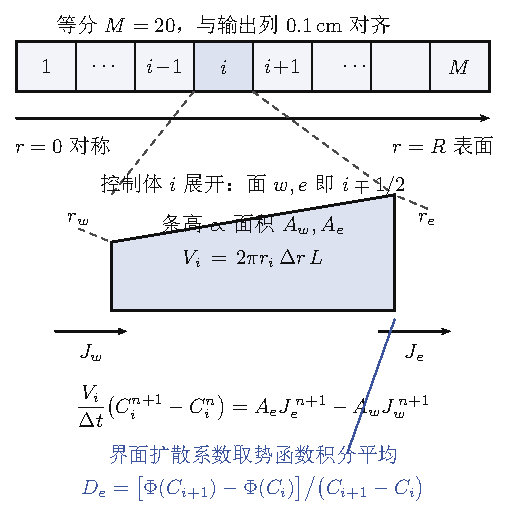
\includegraphics[width=0.8\textwidth,height=0.8\textheight,keepaspectratio]{../figures/tikz_fvm_mesh.pdf}
  \caption{有限体积网格：节点、控制面与环形控制体上的进出通量平衡}
  \label{fig:tikz_fvm_mesh}
\end{figure}

图~\ref{fig:tikz_fvm_mesh} 显示每个控制体的净储量变化等于其两侧控制面的通量差，逐控制体
求和后内部通量成对抵消，只剩表面对流项，从而在离散层面精确复现连续守恒律。这一守恒性
在第\ref{sec:verify}节被量化为 $10^{-13}\sim10^{-16}$ 量级的机器精度残差。

\subsection{界面扩散系数的 Kirchhoff 积分平均}\label{sub:kirchhoff}

式~\eqref{eq:fvm} 需要控制面处的等效扩散系数 $\widehat{D}_{j\pm1/2}$。由于 $D(C)$ 随 $C$ 跨越
约一个数量级（图~\ref{fig:diffusivity_range}），常用的算术平均会高估、调和平均会被最小值
锁死。为在界面处保持通量 $D\,\partial_r C=\partial_r\Phi(C)$ 的一致性，引入 Kirchhoff 势
$\Phi(C)=\int^{C} D(s)\,\mathrm{d}s$\upcite{gama2021,ramos2024}。对 Arrhenius 型
式~\eqref{eq:diff} 的含水率因子解析积分得
\begin{equation}\label{eq:kirchhoff}
\Phi(C)=C\,e^{-a/C}-a\,E_1\!\left(\frac{a}{C}\right),\qquad
\widehat{D}_{j+\frac12}=\frac{\Phi(C_{j+1})-\Phi(C_j)}{C_{j+1}-C_j},
\end{equation}
其中 $E_1(\cdot)$ 为指数积分函数，数值上按其标准级数与渐近展开求值。式~\eqref{eq:kirchhoff}
的界面平均保证了跨界面扩散通量守恒，其对达标时刻的影响见图~\ref{fig:interface_scheme}
与第\ref{sec:sens}节：改用算术平均仅使 $t^*$ 变化 $-1.80\%$，而调和平均因被
最小值锁死产生 $557.76\,\mathrm{h}$ 的非物理结果。

\begin{figure}[H]
  \centering
  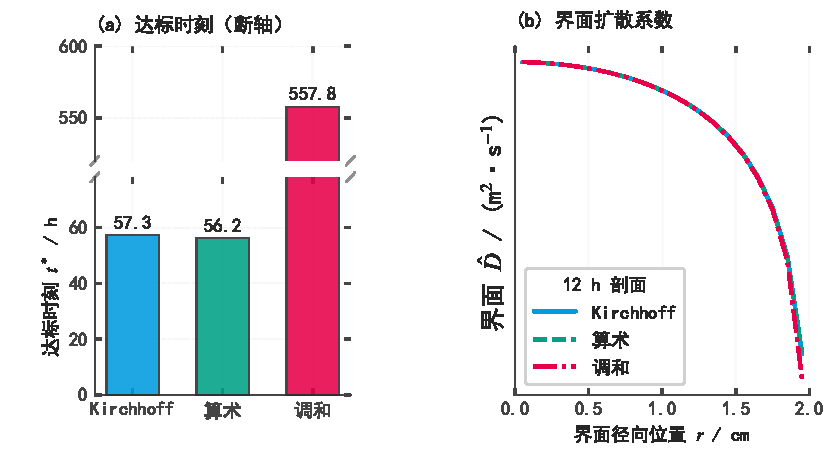
\includegraphics[width=0.9\textwidth,height=0.8\textheight,keepaspectratio]{../figures/fig_interface_scheme.pdf}
  \caption{界面扩散系数平均方式（Kirchhoff、算术、调和）对达标时刻的影响}
  \label{fig:interface_scheme}
\end{figure}

图~\ref{fig:interface_scheme} 直观显示调和平均在 $D$ 跨量级处严重偏离，而 Kirchhoff 积分平均
与算术平均接近且更符合通量守恒，故全文界面扩散系数统一采用式~\eqref{eq:kirchhoff}。

\subsection{时间推进：后向 Euler 与 Picard 内迭代}

物性 $\rho,c_p,k,D$ 依赖待求的 $T,C$，式~\eqref{eq:fvm} 是强非线性刚性方程组。为兼顾稳定性
与守恒性，采用 $L$-稳定的后向 Euler 格式（$\theta=1$），并在每个时间步用 Picard 迭代把
非线性物性冻结更新\upcite{blasik2015}：
\begin{equation}\label{eq:picard}
\frac{\mathbf{U}^{n+1,(m+1)}-\mathbf{U}^{n}}{\Delta t}
=\mathcal{L}\!\big(\mathbf{U}^{n+1,(m)}\big)\,\mathbf{U}^{n+1,(m+1)},
\qquad
\big\|\mathbf{U}^{(m+1)}-\mathbf{U}^{(m)}\big\|_\infty<\varepsilon ,
\end{equation}
其中 $\mathbf{U}=(T,C)$ 在\textbf{同一}迭代回路内联立更新以保持双向耦合，$\mathcal{L}$ 为
按上一迭代场组装的三对角算子，收敛容差 $\varepsilon=10^{-11}$、最大迭代 40 次。实测每步
Picard 残差降至 $9.998\times10^{-12}$（表~\ref{tab:verification}）。此外，Arrhenius 项在
Kelvin 下计算并施加 $200<T_K<500$ 的物理性断言，避免温度越界导致的数值发散。

至此，公共内核（守恒律—有限体积—Kirchhoff 界面—后向 Euler/Picard）建立完毕。以下四章
分别说明各问在此内核上的具体设定与结果。
